
<<<<<<< HEAD
We tried to find a dataset with handwritten text at the beginning of the project, but it turns out there are not that many available. 
% Not sure what Image is supposed to be referenced here.
The datasets that do exist, like following image example. See Figure {figure: wordsexamples}, they would have needed a lot of preprocessing before we could use them in our project.
We would have had to implement baseline slant normalization, skew correction, skeleton and so on.
=======
An attempt was made to find a dataset with handwritten text, but no dataset that fulfilled our requirements was found.
The datasets that were found would require a lot of preprocessing. 
Figure~\ref{} shows a sample from that kind of dataset.
To get good result from that kind of dataset it would be necessary to implement baseline slant normalization, skew correction, skeleton and so on.
>>>>>>> 948876770f033e08bd8f68f88f1f7bb0debc7a02

Therefore, instead of spending a lot of time preprocessing the datasets, we implemented a Graphical User Interface to create our own dataset.
The largest advantages of this solution is that our solution records one pixel wide lines and the characters are already separated. 
The large part of the work, image processing, was thus reduced significantly.
Our dataset contains 100 examples for every capital letter in the Latin alphabet
\footnote{The dataset is available together with the source code of the system. See appendix~\ref{app:source_code}.}.
An example image from our character image dataset can be found in Figure~\ref{fig:image_feature_extraction}.

<<<<<<< HEAD


Furthermore, if the vocabulary is relatively large, we found that it became easier for us to test the HMM.
This is because our word training data is made up of randomly chosen samples.
=======
To get a dataset for training the word classifier a generator was created\footnote{Please, see HandReco\/src\/api\/word\_examples\_generator.py in the source code for documentation of the word example generator. See appendix~\ref{app:source_code}.}.
The generator creates random errors in the words given as input.
To generate the dataset is obviously not optimal for practical applications, but it is good enough to test the implementation.
>>>>>>> 948876770f033e08bd8f68f88f1f7bb0debc7a02

\begin{figure}[h!]
  \centering
  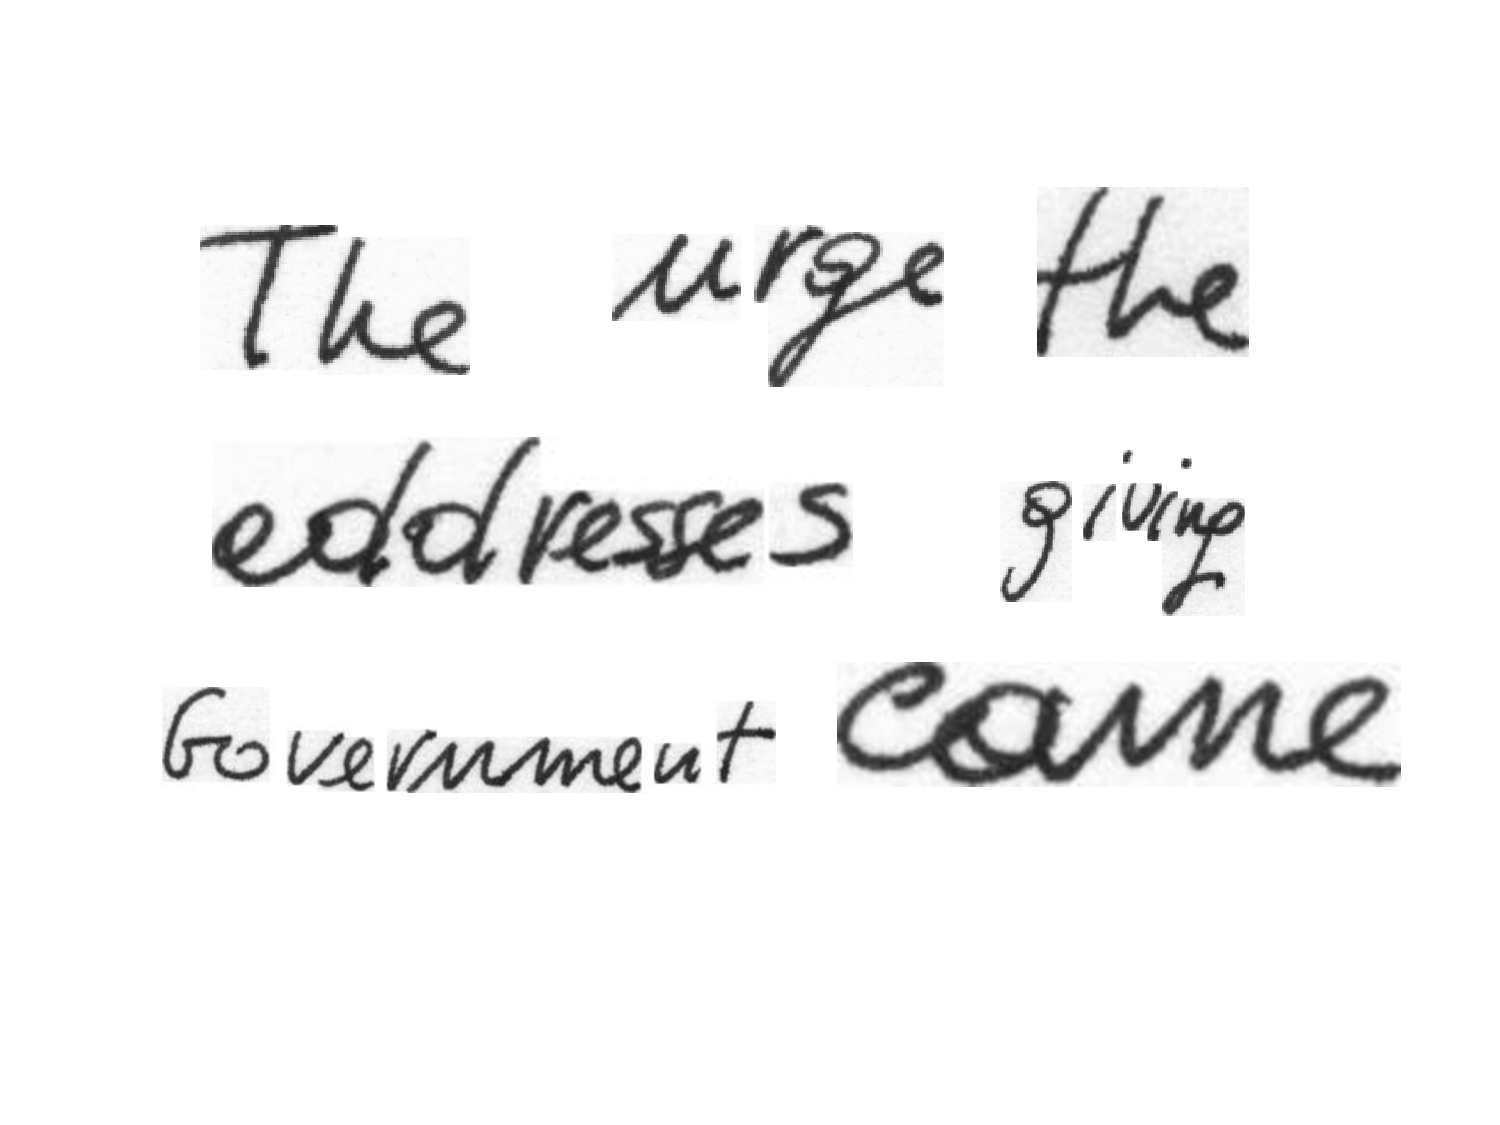
\includegraphics[width=5in]{datasets_examples}
  \caption{Word image examples}
  \label{figure:wordsexamples}
\end{figure}
